
\chapter{Adquisición y limpieza de los datos}\label{chap:adq}

En cualquier proyecto de Data Science es necesario trabajar con una cantidad relativamente grande de datos. Sin embargo, normalmente el estado y el formato en el que se encuentran los datos de los que puede disponerse en Internet no se adecúan a las necesidades concretas del proyecto. Además, es habitual encontrar fuentes de datos con un número elevado de campos; es también tarea de esta etapa obtener los campos necesarios para el proyecto con el fin de aligerar las ejecuciones, ya que la mayoría de modelos son sensibles a la cantidad de campos. Por tanto, el proceso de adquisición y limpieza de los datos se convierte en una parte muy importante del proceso. Los objetivos principales de la etapa de limpieza de los datos son los siguientes:
\begin{itemize}
    \item Adaptar el formato a los requerimientos del proyecto.
    \item Eliminar registros incorrectos.
    \item Completar registros en los que falte alguno de los datos.
    \item Dejar únicamente los campos necesarios para el proyecto a desarrollar.
\end{itemize}

Para la creación del sistema de recomendación de películas basado en contenido que se desarrollará en este proyecto se utilizará un dataset consistente en información sobre varios miles de películas disponible en \cite{kaggle}. El dataset consiste en dos ficheros: películas y créditos. Los campos disponibles en los ficheros son los siguientes:

\begin{itemize}
    \item Películas
    \begin{itemize}
        \item budget: Presupuesto de la película en Dólares.
        \item genres: Generos cinematográficos asociados a la película.
        \item homepage: Página web de la productora de la película.
        \item id: Identificador único dentro del dataset.
        \item plot\_keywords: Palabras clave.
        \item original\_language: Idioma original
        \item original\_title: Título original de la película
        \item overview: Resumen
        \item popularity: Popularidad (unidades desconocidas)
        \item production\_companies: Compañías encargadas de la producción
        \item production\_countries: Paises productores de la película
        \item release\_date: Fecha de lanzamiento de la película
        \item revenue: Recaudación de la película en dólares
        \item runtime: Días en cartelera
        \item spoken\_languages: Idiomas hablados en la película
        \item status: Estado de la película
        \item tagline: Subtítulo
        \item title: Título en inglés
        \item vote\_average: Promedio de votos en IMDB
        \item vote\_count: Número de votos en IMDB
    \end{itemize}
    \item Créditos
    \begin{itemize}
        \item movie\_id: Identificador de la película (para unirlo con el dataset anterior).
        \item title: Título en inglés de la película
        \item cast: Actores que aparecen (en orden e importancia). Campo en formato JSON.
        \item crew: Equipo participante en la película, es un JSON con una lista de diccionarios. Cada elemento de la lista tiene el nombre del participante y el cargo.
    \end{itemize}
\end{itemize}

En la \autoref{tab:peliculas} puede verse un análisis descriptivo de los campos numéricos de los datos anteriormente mencionados. El resto de campos son campos de texto:

\begin{table}[h]
\centering
\resizebox{0.8\textwidth}{!}{%
\begin{tabular}{lrrrrrrr}
\toprule
{} &        budget &   popularity &       revenue &      runtime &  vote\_average &    vote\_count \\
\midrule
count &  $4.8\cdot 10^{3}$ &  $4803.0$ &  $4.8\cdot 10^{3}$ &  $4801.0$ &   $4803.0$ &   $4803.0$ \\
mean  &  $2.9\cdot 10^{7}$ &   $21.5$ &  $8.2\cdot 10^{7}$ &   $106.9$ &      $6.1$ &    $690.2$ \\
std   &  $4.1\cdot 10^{7}$ &   $31.8$ &  $1.6\cdot 10^{8}$ &    $22.6$ &      $1.2$ &   $1234.5$ \\
min   &  $0.0\cdot 10^{0}$ &       $0.0$ &  $0.0\cdot 10^{0}$ &     $0.0$ &      $0.0$ &      $0.0$ \\
25\%   &  $7.9\cdot 10^{5}$ &    $4.7$ &  $0.0\cdot 10^{0}$ &    $94.0$ &      $5.6$ &     $54.0$ \\
50\%   &  $1.5\cdot 10^{7}$ &   $12.9$ &  $1.9\cdot 10^{7}$ &   $103.0$ &      $6.2$ &    $235.0$ \\
75\%   &  $4.0\cdot 10^{7}$ &   $28.3$ &  $9.3\cdot 10^{7}$ &   $118.0$ &      $6.8$ &    $737.0$ \\
max   &  $3.8\cdot 10^{8}$ &  $875.6$ &  $2.8\cdot 10^{9}$ &   $338.0$ &     $10.0$ &  $13752.0$ \\
\bottomrule
\end{tabular}}
\caption{Análisis descriptivo de las variables numéricas de los datos de entrada. Se muestra para cada campo el número de filas informadas, la media, la desviación estándar y los cuartiles.}
\label{tab:peliculas}
\end{table}

\newpage
\section{Importación de datos de películas}

El primer paso en la etapa de adquisición de los datos consiste en leer ambos ficheros (en formato csv) y obtener los DataFrame de Pandas correspondientes. Las columnas genres, keywords, production\_countries, production\_companies, spoken\_languages, cast y crew están en formato json en origen. Es por ello que en las funciones de lectura de los datos tienen un trato especial. Las funciones implementadas son las siguientes:

\begin{lstlisting}[language=Python, caption={Lectura de los datos del fichero de películas. Se carga el fichero desde la ruta y se mapea la fecha de lanzamiento a un objeto de tipo fecha.}]
import json
import pandas as pd
def carga_peliculas(ruta):
    """Función utilizada para cargar el dataset de las películas. Se transforma a fecha el campo de fecha de salida
    y se cargan como listas los campos que están guardados como json.
    Args:
        ruta (str): Ruta hasta el archivo de tmdb_5000_peliculas.csv
    Returns:
        pd.DataFrame: Dataframe de pandas con la información del csv
    """
    df = pd.read_csv(ruta)
    df['release_date'] = pd.to_datetime(df['release_date']).apply(lambda x: x.date())
    json_columns = ['genres', 'keywords', 'production_countries', 'production_companies', 'spoken_languages']
    for columna in json_columns:
        df[columna] = df[columna].apply(json.loads)
    return df
\end{lstlisting}

\begin{lstlisting}[language=Python, caption={Lectura de los datos del fichero de créditos. Se carga el fichero desde la ruta dada.}]
def carga_creditos(ruta):
    """Función utilizada para cargar el dataset de los créditos. Se cargan como listas los campos que están guardado
    Args:
        ruta (str): Ruta hasta el archivo de tmdb_5000_creditos.csv
    Returns:
        pd.DataFrame:
    """
    df = pd.read_csv(ruta)
    json_columns = ['cast', 'crew']
    for columna in json_columns:
        df[columna] = df[columna].apply(json.loads)
    return df
\end{lstlisting}

Pandas es una librería rápida, flexible, opensource y relativamente fácil de usar. Está implementada en Python y es una de las librerías más usadas para realizar tareas de análisis y manipulación de datos. En este proyecto esta librería será utilizada de forma extensiva. Con estas dos funciones se consigue tener los datos en el tipo de dato que proporciona Pandas, el DataFrame. Este tipo de objeto tiene formato tabular (donde una fila es un registro y una columna un atributo del registro) y tiene multitud de métodos implementados para la transformación de datos.\\

En esta primera etapa de importación, el objetivo es obtener un único DataFrame que contenga información de ambos conjuntos de datos. Un problema habitual que tiene lugar al juntar dos ficheros es la información faltante de los ficheros. Hay que tratar de forma especial el acceso a los datos de cada DataFrame a la hora de juntarlos, pues puede que haya campos que no estén informados. Para ello, definimos una función que accede de forma segura a los datos, ya que en caso de no encontrarlo devuelve nulo, evitando errores de ejecución.

\begin{lstlisting}[language=Python, caption={Acceso a los datos de forma segura. Se utiliza como proxy para no acceder directamente al valor. De esta forma, si se da un error, en vez de tener un error de ejecución se devuelve nulo.}]
def get_elemento(contenedor, valores_indice):
    """Función para acceder de forma segura a valores. En caso de que no se encuentre uno de ellos, se devuelve NaN
    en vez de lanzar un error.
    Args:
        contenedor (list): Lista/ contenedor de la que quieren extraerse los valores
        valores_indice (list): Lista de índices a extraer del contenedor
    Returns:
        any: Valores extraidos
    """
    result = contenedor
    try:
        for idc in valores_indice:
            result = result[idc]
        return result
    except IndexError or KeyError:
        return pd.np.nan
\end{lstlisting}

Uno de los campos a extraer del fichero de créditos es el de director. Este campo se encuentra dentro del campo de crew (en formato json) con la clave director. Por tanto, para añadirlo al DataFrame es necesario buscarlo. Para ello se define la función get\_director.
\begin{lstlisting}[language=Python, caption= {Obtención de una lista de directores extraídos del campo crew. Se itera por todos los miembros del equipo y se retienen únicamente aquellos que tienen el cargo de director.}]
def get_director(datos_equipo):
    """Devuelve el director dado un json con toda la composición del equipo de la película.
    Args:
        datos_equipo (json): JSON con el equipo que ha realizado la película
    Returns:
        str: Director de la película
    """
    directores = [x['name'] for x in datos_equipo if x['job'] == 'Director']
    return get_elemento(directores, [0])
\end{lstlisting}

Como se ha visto anteriormente, el objetivo del proyecto es crear un sistema de recomendación de películas basado en contenido. Por tanto, resulta vital conseguir información del contenido de las películas. El campo fundamental para conseguir este fin es el campo keywords, que contiene las palabras clave de cada película. Este campo está en origen en formato JSON, con información que no es relevante para el objetivo del proyecto. Para obtener únicamente las palabras clave se implementa pipe\_flatten\_names que extrae estas palabras clave.
\begin{lstlisting}[language=Python, caption= {Extracción de las palabras clave a partir del JSON del DataFrame. }]
def aplana_nombres(keywords):
    """Obtiene una lista con las keywords separadas por un pipe | extrayéndolas del json.
    Args:
        keywords (json): keywords de la película
    Returns:
        str: keywords de la película juntas
    """
    return '|'.join([x['name'] for x in keywords])
\end{lstlisting}

Para terminar con la etapa de importación y carga de los datos, se crea la función que añade al DataFrame de películas la información de credits necesaria.
\begin{lstlisting}[language=Python, caption= {El conjunto de datos se encuentra en dos ficheros separados y con estructuras diferentes. Se juntan esas dos colecciones un un único conjunto de datos.}]
def combina_colecciones(peliculas, creditos):
    """Aplica una serie de funciones para añadir información al dataset de películas a partir del
    conjunto de datos de créditos
    Args:
        peliculas (pd.DataFrame): DataFrame obtenido de leer el archivo de películas
        creditos (pd.DataFrame): DataFrame obtenido de leet el archivo de créditos
    Returns:
        pd.DataFrame: DataFrame con la información conjunta
    """
    tmdb_peliculas = peliculas.copy()
    tmdb_peliculas.rename(columns=EQUIVALENCIAS_TMDB_IMDB, inplace=True)
    tmdb_peliculas['title_year'] = pd.to_datetime(tmdb_peliculas['release_date']).apply(lambda x: x.year)
    # I'm assuming that the first production country is equivalent, but have not been able to validate this
    tmdb_peliculas['country'] = tmdb_peliculas['production_countries'].apply(lambda x: get_elemento(x, [0, 'name']))
    tmdb_peliculas['language'] = tmdb_peliculas['spoken_languages'].apply(lambda x: get_elemento(x, [0, 'name']))
    tmdb_peliculas['director_name'] = creditos['crew'].apply(get_director)
    tmdb_peliculas['actor_1_name'] = creditos['cast'].apply(lambda x: get_elemento(x, [1, 'name']))
    tmdb_peliculas['actor_2_name'] = creditos['cast'].apply(lambda x: get_elemento(x, [2, 'name']))
    tmdb_peliculas['actor_3_name'] = creditos['cast'].apply(lambda x: get_elemento(x, [3, 'name']))
    tmdb_peliculas['genres'] = tmdb_peliculas['genres'].apply(aplana_nombres)
    tmdb_peliculas['plot_keywords'] = tmdb_peliculas['plot_keywords'].apply(aplana_nombres)
    return tmdb_peliculas
\end{lstlisting}

Por último, se cargan las librerías necesarias para el proyecto y se leen los datos de los ficheros, usando las funciones definidas anteriormente.
\begin{lstlisting}[language=Python, caption=Código usado para la carga de los datos. Se aplican las funciones definidas anteriormente para obtener, a partir de los CSV un único dataframe, que será con el que se trabaje el resto del tiempo]
import numpy as np
import matplotlib as mpl
import matplotlib.pyplot as plt
import seaborn as sns
import math, nltk, warnings
from nltk.corpus import wordnet
from sklearn import linear_model
from sklearn.neighbors import NearestNeighbors
from fuzzywuzzy import fuzz
from wordcloud import WordCloud, STOPWORDS
plt.rcParams["patch.force_edgecolor"] = True
plt.style.use('fivethirtyeight')
mpl.rc('patch', edgecolor = 'dimgray', linewidth=1)
from IPython.core.interactiveshell import InteractiveShell
InteractiveShell.ast_node_interactivity = "last_expr"
pd.options.display.max_columns = 50
%matplotlib inline
warnings.filterwarnings('ignore')

#Definimos la función a utilizar para obtener el lexema de las palabras.
PS = nltk.stem.PorterStemmer()
#__________________
# load the dataset
#df_inicial = pd.read_csv("../input/movie_metadata.csv")
creditos = carga_creditos("../RecommendationEngine/datos/tmdb_5000_credits.csv")
peliculas = carga_peliculas("../RecommendationEngine/datos/tmdb_5000_movies.csv")
df_inicial = combina_colecciones(peliculas, creditos)
\end{lstlisting}

Con esto, se consigue tener un único DataFrame sobre el que trabajar.

\newpage
\section{Limpieza y transformación de los datos}

Una vez se han importado y cargado los datos, la siguiente etapa es el limpiado de los datos, tanto para lidiar con los posibles datos faltantes.

\subsection{Entradas duplicadas}

En ocasiones los datasets que se encuentran en Internet no están en un estado perfecto, y en ocasiones se tienen datos duplicados. Es importante comprobar si existen datos duplicados, ya que si no a la hora de crear modelos puede darse más importancia a unos registros que a otros, lo cual resulta un error de concepto. En primer lugar, por tanto, comprobamos la existencia de entradas duplicadas.
\begin{lstlisting}[language=Python, caption=Entradas duplicadas. Se buscan entradas duplicadas a partir del id de la película y se devuelve la cantidad de películas repetidas.]
entradas_duplicadas = df_inicial[df_inicial.id.duplicated()]
entradas_duplicadas.shape
\end{lstlisting}
El resultado es que no existen entradas duplicadas. Sin embargo, comprobar la duplicidad de esta forma tan genérica puede no solucionar todos los posibles problemas. Por ejemplo, podría haber una entrada con un error ortográfico o con diferencias mínimas. En este caso, cada entrada se corresponde con una película, por lo que tener dos entradas que únicamente difieren en, por ejemplo, el presupuesto, podría considerarse una entrada duplicada. Dado que son datos de películas, buscaremos entradas con el mismo título. 

\begin{lstlisting}[language=Python, caption=Entradas con título duplicado. Se buscan películas que tengan el mismo título, para realizar un análisis y determinar si se trata de entradas duplicadas que hay que filtrar o no.]
df_temp = df_inicial
lista_var_de_duplicados = ['movie_title', 'title_year', 'director_name']
lista_duplicados = df_temp['movie_title'].map(df_temp['movie_title'].value_counts() > 1)
df_temp[lista_duplicados][lista_var_de_duplicados].sort_values('movie_title')
\end{lstlisting}

El resultado se muestra en la \autoref{tab:duplicated_entries}. Como puede comprobarse, únicamente hay tres parejas de películas con el mismo título. Analizándolo a simple vista puede verse que se trata de remakes, por lo que no podemos considerarlo como entradas duplicadas, ya que pueden diferir en calidad e incluso en alguna palabra clave.\\

\begin{table}[h]
\centering
\begin{tabular}{llrl}
\toprule
\textbf{id} &     \textbf{movie\_title} &  \textbf{title\_year} &        \textbf{director\_name} \\
\midrule
1359 &           Batman &      1989 &           Tim Burton \\
4267 &           Batman &      1966 &  Leslie H. Martinson \\
3647 &  Out of the Blue &      1980 &        Dennis Hopper \\
3693 &  Out of the Blue &      2006 &       Robert Sarkies \\
972  &         The Host &      2013 &        Andrew Niccol \\
2877 &         The Host &      2006 &         Bong Joon-ho \\
\bottomrule
\end{tabular}
\caption{Entradas con el título duplicado. Puede verse que se no se trata de una errata, ya que aunque las películas se llaman igual, son de años diferentes y tienen directores diferentes. Esto significa que, probablemente, se trate de \textit{remakes} de las películas originales.}
\label{tab:duplicated_entries}
\end{table}

Por tanto, puede concluirse que en el dataset no existen entradas duplicadas. A pesar de tener el mismo dataset al inicio de este apartado que ahora, se ha incluido por completitud, ya que es un paso que debe realizarse siempre.

\subsection{Limpieza de las keywords de las películas}

Las keywords tendrán un papel fundamental en el funcionamiento del sistema. De hecho, como se verá en el \autoref{chap:creacion}, las recomendaciones se realizarán en base a la similaridad entre películas, y para esta medida se usarán las keywords. Por tanto, se hace necesario analizar el contenido de esta variable, puesto que se realizará un uso extensivo de ella.\\

Inicialmente, el dataset contiene un total de 9474 keywords. En la \autoref{fig:keywords_histogram} se muestra la distribución del número de keywords. Puede verse que aun habiendo casi el doble de keywords que de películas, la mayoría de películas contienen entre 5 y 15 keywords, por lo que el número de keywords no es preocupante.
\begin{figure}[H]
    \centering
    \captionsetup{width=10cm}
    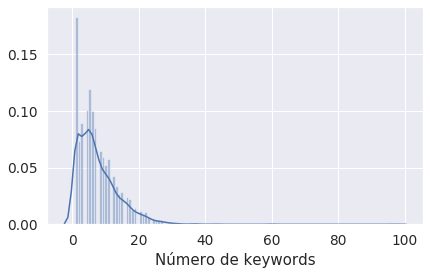
\includegraphics[width=12cm]{contenido/imagenes/keyword_histogram.png}
    \caption{Histograma con el número de keywords de cada película.}
    \label{fig:keywords_histogram}
\end{figure}

Sin embargo, tratar con lenguaje natural siempre implica poner especial atención en lo que se consideran palabras diferentes. Es lógico pensar que a la hora de poner las keywords de las películas no se ha tenido en cuenta las posibles similitudes entre keywords ni se han asignado de una lista cerrada.\\

Los seres humanos nos expresamos de forma muy diferente y probablemente las keywords hayan sido asignadas por personas diferentes. Por lo cual es esperable que haya keywords que signifiquen aproximadamente lo mismo pero que por tener distintas grafías actualmente se considerarían diferentes palabras.\\

El lenguaje de Python es ampliamente utilizado en la disciplina de la ciencia de datos, es por ello que existen numerosas librerías de inestimable ayuda para el NLP. Una de las más conocidas es NLTK \cite{NLTK} (\textbf{N}atural \textbf{L}anguage \textbf{T}ool\textbf{K}it).\\

En este proyecto es importante extraer el significado original de las keywords, es decir, no importa si la keyword es ``drama'' o ``dramático'', ya que significan lo mismo. En este caso utilizamos la librería NLTK, que en concreto implementa una función denominada \texttt{PorterStemmer}\cite{porter}, que es una función que sirve para extraer lexemas de las palabras. Con este paso se consigue extraer la raíz de la palabra para evitar problemas con plurales, etc. En primer lugar se implementa la función\texttt{keywords\_inventory} que recoge las keywords y crea un diccionario para ver en qué palabra queda otra.

\begin{lstlisting}[language=Python, caption= Obtención del lexema de cada keywords y creación del diccionario de equivalencia. Se itera sobre cada una de las películas y se extraen sus palabras clave. Para evitar palabras derivadas con el mismo significado, se extrae y se almacena el lexema de cada keyword.]
def inventario_keywords(dataframe, columna = 'plot_keywords'):
    """Devuelve un diccionario con las palabras que derivan de cada lexema
    a partir de un DataFrame y la columna de la que se quiere extraer
    Args:
        dataframe (pd.DataFrame): DataFrame del que obtener la información.
        columna (str, optional): Nombre de la columna. Por defecto 'plot_keywords'.
    Returns:
        list: Keywords finales que aparecen
        dict: Relación lexema <-> palabras
        dict: Palabra más corta derivada del lexema
    """
    PS = nltk.stem.PorterStemmer()
    keywords_raices  = dict()  # recoger las palabras de cada lexema
    keywords_selecciona = dict()  # asociacion: lexema <-> keyword
    category_keys = []
    icuenta = 0
    for s in dataframe[columna]:
        if pd.isnull(s): continue
        for t in s.split('|'):
            t = t.lower()
            raiz = PS.stem(t)
            # Para cada lexema, un set con las palabras que lo usan
            if raiz in keywords_raices:                
                keywords_raices[raiz].add(t)
            else:
                keywords_raices[raiz] = {t}
    
    for s in keywords_raices.keys():
        if len(keywords_raices[s]) > 1:  
            longtud_min = 1000
            for k in keywords_raices[s]:
                if len(k) < longtud_min:
                    clave = k ; longtud_min = len(k)            
            category_keys.append(clave)
            keywords_selecciona[s] = clave
        else:
            category_keys.append(list(keywords_raices[s])[0])
            keywords_selecciona[s] = list(keywords_raices[s])[0]
                   
    print("Número de keywords en la variable: '{}': {}".format(columna,len(category_keys)))
    return category_keys, keywords_raices, keywords_selecciona
\end{lstlisting}

Con el fin de limpiar el dataset se implementa la función \texttt{df\_keywords\_replacement}. Algunos cambios que realiza este paso es tomar por iguales orc y orcs, spy y spying o time travel y time traveler.
\begin{lstlisting}[language=Python, caption= Extracción del lexema de las keywords. Reemplaza las apariciones de una palabra clave por su lexema, con el fin de extraer el significado de la palabra clave y reducir su cantidad.]
def df_reemplazo_keywords(df, dicc_reemplazo, raiz = False, columna = 'plot_keywords'):
    """Reemplaza las palabras clave de una película por las formas básicas de las mismas.
    Args:
        df (pd.DataFrame): DataFrame que contiene la información de las películas
        dicc_reemplazo (dict): Diccionario con los cambios
        raiz (bool, optional): Controla si se obtienen las raices de las palabras de las
        keywords. Por defecto False.
        columna (str, optional): Columna en la que realizar la transformación. Por defecto 'plot_keywords'.
    Returns:
        pd.DataFrame: DataFrame con las sustituciones realizadas
    """
    PS = nltk.stem.PorterStemmer()
    df_nuevo = df.copy(deep = True)
    for indice, fila in df_nuevo.iterrows():
        cadena = fila[columna]
        if pd.isnull(cadena): continue
        nueva_lista = []
        for s in cadena.split('|'): 
            clave = PS.stem(s) if raiz else s
            if clave in dicc_reemplazo.keys():
                nueva_lista.append(dicc_reemplazo[clave])
            else:
                nueva_lista.append(s)       
        df_nuevo.at[indice, columna] = '|'.join(nueva_lista)
    return df_nuevo
\end{lstlisting}

Finalmente, se realiza el cambio en el dataset de la siguiente manera:

\begin{lstlisting}[language=Python, caption= Sustitucion de las keywords por su forma primitiva.]
keywords, keywords_roots, keywords_select = keywords_inventory(df_duplicate_cleaned,
                                                               column = 'plot_keywords')
df_keywords_cleaned = df_keywords_replacement(df_duplicate_cleaned, keywords_select,
                                               roots = True)
\end{lstlisting}

\subsection{Sinónimos}

En la sección anterior de la memoria, se han explicado las peculiaridades de trabajar con un dataset que contenga texto, así como la estrategia seguida par reducir la cantidad de keywords. Sin embargo, únicamente hemos agrupado las keywords por su lexema, que es además la forma más simple de realizar esta agrupación. Por ejemplo, si hubiera dos películas, una con la keyword alien y otra con la keyword extraterrestre, únicamente con el paso anterior seguirían siendo películas diferentes.\\

En esta sección se va un paso más allá. La librería NLTK además de extractores de lexema, incluye un submódulo de corpus. En este caso se utilizará el corpus de WordNet. Consiste en una base de datos léxica de sustantivos, verbos, adjetivos y adverbios en inglés agrupados en conjuntos de sinónimos cognitivos, expresando cada uno un concepto diferente. Se trata de una herramienta con muchísimo potencial para el análisis de texto.\\

En este caso concreto, se utilizará el corpus de WordNet \cite{WordNet} implementado en la librería NLTK para sustituir las keywords con menos apariciones por sus sinónimos más frecuentes. Por ejemplo, la keyword extraterrestrial aparece un total de 4 veces. Es posible que sustituirla por alien en esas 4 películas haga que las películas de aliens estén mejor relacionadas, ya que no hay apenas diferencia entre los significados. En concreto, las keywords con menos de 5 apariciones serán sustituidas por su sinónimo más frecuente. Con esto se reemplaza aproximadamente el $6 \%$ de las keywords.
\begin{lstlisting}[language=Python, caption= Sustitución de las palabras menos frecuentes por sus sinónimos. En este caso, puede ser un problema el tener palabras dfierentes con el mismo significado, ya que podría enmascarar relaciones entre películas. Para ello, se buscan los sinónimos de las keywords y se sustituye la keyword por el sinónimo con mayor número de apariciones.]
def prueba_keyword(palabra, keyword_apariciones, umbral):
    """Devuelve si una palabra aparece un número mayor de veces que el umbral señalado
    Args:
        palabra (str): Palabra a buscar
        keyword_apariciones (dict): Diccionario con las apariciones de cada keyword
        umbral (int): Umbral
    Returns:
        bool: True si aparece un número mayor de veces
    """
    return (False , True)[keyword_apariciones.get(palabra, 0) >= umbral] 

veces_keyword.sort(key = lambda x:x[1], reverse = False)
keyword_cuenta = dict()
for s in veces_keyword:
    keyword_cuenta[s[0]] = s[1]
# Creación de un diccionario para reemplazar keywords por sinónimos de mayor frecuencia
palabra_reemplazo = dict()
icuenta = 0
for _, [palabra, num_apariciones] in enumerate(veces_keyword):
    if num_apariciones > 5:
        continue  # Sólo las keywords que aparecen menos de 5 veces
    lexema = toma_sinonimos(palabra)
    if len(lexema) == 0:
        continue     #Caso de plurales
    lista_palabras = [(s, keyword_cuenta[s]) for s in lexema 
                  if prueba_keyword(s, keyword_cuenta, keyword_cuenta[palabra])]
    lista_palabras.sort(key = lambda x:(x[1],x[0]), reverse = True)    
    if len(lista_palabras) <= 1:
        continue       # NO se reemplaza
    if palabra == lista_palabras[0][0]:
        continue    # Reemplazo por sí mismo
    icuenta += 1
    if  icuenta < 8:
        print('{:<12} -> {:<12} (inic: {})'.format(palabra, lista_palabras[0][0], lista_palabras))
    palabra_reemplazo[palabra] = lista_palabras[0][0]
\end{lstlisting}

Conviene recordar que el objetivo de este proyecto es crear un sistema de recomendación de películas \textbf{basado en contenido}. Por ello, de poco sirve tener una keyword que aparezca en una cantidad muy reducida de películas.

\begin{figure}[H]
    \centering
    \captionsetup{width=12cm}
    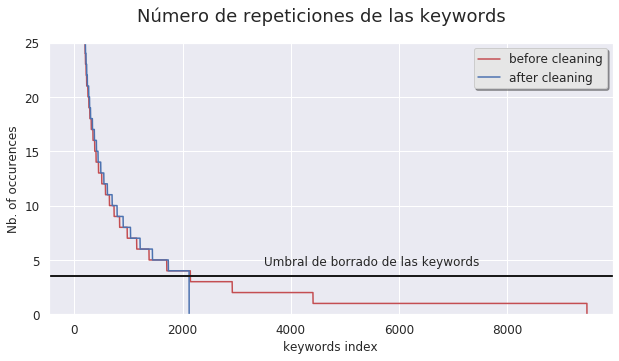
\includegraphics[height=9.3cm]{./contenido/imagenes/keyword_cleaning.png}
\caption{Repeticiones de las keywords antes y después de la limpieza.}
\label{fig:key_cleaning}
\end{figure}

En este caso se ha decidido eliminar las keywords con menos de $3$ repeticiones, que como puede verse en la \autoref{fig:key_cleaning} afecta a la mayoría de keywords, pasando a tener aproximadamente $6500$ keywords menos. Puede parecer que perdemos mucha información, pero lo que se busca es tener relaciones potentes. Además, como se verá más adelante, se definirá una distancia entre películas, por lo que no es conveniente tener demasiadas dimensiones, ya que se podría tener el problema de la dimensionalidad \cite{wiki:CurseOfDimensionality}

\newpage
\section{Imputación de valores faltantes}

En estadística, la imputación es el proceso de reemplazar los datos faltantes con valores sustitutos. Son tres los principales problemas que causan los datos faltantes:
\begin{itemize}
    \item Introducir una cantidad sustancial de bias.
    \item Hacer más complicado el tratamiento de los datos.
    \item Empeorar la eficiencia de los modelos.
\end{itemize}

Siempre es interesante realizar un análisis de las entradas que tienen datos faltantes, ya que por ejemplo si se tuviera un dataset con información de varias estaciones de medición, podría ser que los datos faltantes no fueran aleatorios, sino producidos por una situación concreta de alguna de las estaciones.\\

Existen dos técnicas principales para imputar estos datos:

\begin{itemize}
    \item Sustitución promedio: Implica reemplazar los valores faltantes con la media de esa variable en los demás casos. Tiene el beneficio de no cambiar la media de la distribución. Sin embargo, atenúa las correlaciones que implican a la variable imputada.
    \item Imputación mediante regresión: Es, por así decirlo, la forma opuesta de realizar la imputación. Imputa una de las variables fijándose en una o varias de las demás. En este caso no se genera cambio en la correlación entre variables pero sí se afecta a la media. Otro problema es que supone que la regresión no tiene un término de error asociado y que es, por tanto, una regresión con $R² = 1$.
\end{itemize}

En la \autoref{fig:correlation} se muestra la matriz de correlación entre las variables del dataset, lo cual aporta información sobre qué variables usar para predecir otras.

\begin{figure}[H]
    \centering
    \captionsetup{width=12cm}
    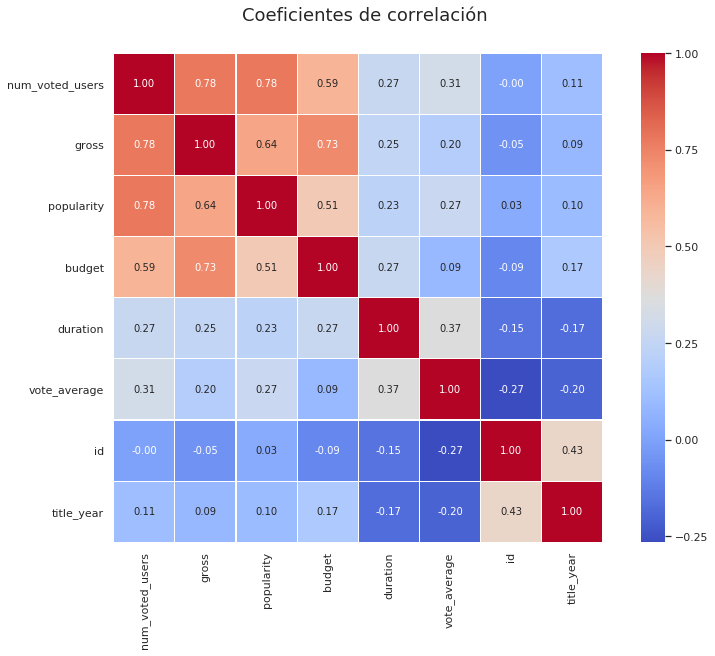
\includegraphics[height=10cm]{./contenido/imagenes/correlation.png}
\caption{Correlación entre las variables del dataset. La matriz es simétrica, ya que la correlación entre A y B es igual que la correlación entre B y A.}
\label{fig:correlation}
\end{figure}

En este caso, se utilizarán varios tipos de imputación, algunos adecuados al dominio concreto del problema. Es necesario resaltar que únicamente se imputarán aquellas variables que sean necesarias para la creación propiamente dicha del recomendados. En la \autoref{fig:completion} se muestran los porcentajes de completitud de cada una de las variables que restan.

\begin{figure}[H]
    \centering
    \captionsetup{width=12cm}
    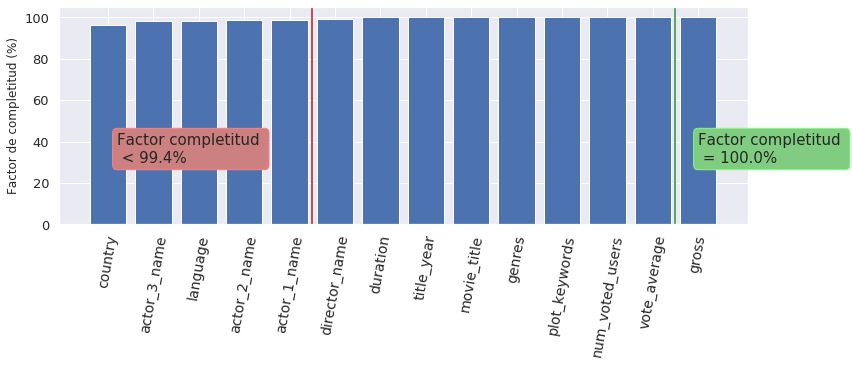
\includegraphics[width= 13cm]{./contenido/imagenes/completion.png}
\caption{Completitud de las variables del dataset. La mayoría de variables tienen un factor de completitud bastante grande.}
\label{fig:completion}
\end{figure}


\subsection{Años faltantes}

En el sistema de recomendación, la variable año se utilizará para recomendar al usuario películas relativamente coetáneas a la dada por el usuario. Con el fin de tener el año informado en la mayor cantidad posible de registros, se completará el año teniendo en cuenta los años de creación del resto de películas de su director y los 3 actores principales, realizando un promedio entre todos ellos. Con este fin se implementa la función \texttt{fill\_year}.

\begin{lstlisting}[language=Python, caption={Completado de la variable año en el dataset utilizando el promedio de los años de las películas de su director y actores principales.}]
def rellena_ano(df):
    """Completa la columna faltante del año teniendo en cuenta la media
    de los periodos de actividad de los actores y el director.
    """
    col = ['director_name', 'actor_1_name', 'actor_2_name', 'actor_3_name']
    ano_habitual = [0 for _ in range(4)]
    var = [0 for _ in range(4)]
    # Año medio de actividad para los actores y el director
    for i in range(len(col)):
        ano_habitual[i] = df.groupby(col[i])['title_year'].mean()
    # Diccionario que recoja esta información
    ano_actor = dict()
    for i in range(4):
        for s in ano_habitual[i].index:
            if s in ano_actor.keys():
                if pd.notnull(ano_habitual[i][s]) and pd.notnull(ano_actor[s]):
                    ano_actor[s] = (ano_actor[s] + ano_habitual[i][s])/2
                elif pd.isnull(ano_actor[s]):
                    ano_actor[s] = ano_habitual[i][s]
            else:
                ano_actor[s] = ano_habitual[i][s]
        
    # Identificación de los años faltantes
    missing_year_info = df[df['title_year'].isnull()]
    # Completado de los valores faltantes
    icuenta_reemplazos = 0
    for indice, fila in missing_year_info.iterrows():
        valor = [ np.NaN for _ in range(4)]
        icuenta = 0 ; suma_ano = 0
        for i in range(4):            
            var[i] = df.loc[indice][col[i]]
            if pd.notnull(var[i]): valor[i] = ano_actor[var[i]]
            if pd.notnull(valor[i]): icuenta += 1 ; suma_ano += ano_actor[var[i]]
        if icuenta != 0: 
            suma_ano = suma_ano / icuenta 
        if int(suma_ano) > 0:
            icuenta_reemplazos += 1
            df.at[indice, 'title_year'] = int(suma_ano)
            if icuenta_reemplazos < 10: 
                print("{:<45} -> {:<20}".format(df.loc[indice]['movie_title'],int(suma_ano)))
    return
\end{lstlisting}


\subsection{Completado de keywords}

Al tratarse de un recomendador basado en contenido, una película que no tenga ninguna keyword nunca será recomendada, ya que no se considerará similar a ninguna. A pesar de que como se ha visto los sistemas basados en contenido y no en opiniones no presentan el problema de los nuevos productos, si que si un producto está ``muerto'' por no tener keywords, lo estará siempre.\\

Para resolver el problema que podría suponer tener películas sin palabras clave, se imputarán keywords en las películas teniendo en cuenta su título. Por ejemplo si la película Alien Covenant no tiene keywords, se incluiría alien como keyword por estar en su título y ser ya una keyword existente. Mediante el \autoref{lst:keywords} se logra la imputación en el DataFrame.

\begin{lstlisting}[language=Python, caption={Imputación de keywords a partir del título de la película. Cuando una película no tiene keywords se utiliza su título como fuente de keywords, tomando del mismo las palabras que ya sean keywords de otra película.}, label ={lst:keywords}]
icuenta = 0
for indice, fila in df_rellenado[df_rellenado['plot_keywords'].isnull()].iterrows():
    icuenta += 1
    lista_palabras = fila['movie_title'].strip().split()
    nueva_keyword = []
    for s in lista_palabras:
        lexema = toma_sinonimos(s)
        for t in list(lexema):
            if t in keywords: 
                nueva_keyword.append(t)                
    if nueva_keyword and icuenta < 15: 
        print('{:<50} -> {:<30}'.format(fila['movie_title'], str(nueva_keyword)))
    if nueva_keyword:
        df_rellenado.at[indice, 'plot_keywords'] = '|'.join(nueva_keyword)
\end{lstlisting}

\subsection{Completado mediante regresiones}

Como puede verse en la \autoref{fig:correlation} hay variables bastante correlacionadas, como la recaudación y el número de usuarios que votaron una película. Esto se entiende porque normalmente las películas con mayor presupuesto son también las que más invierten en marketing. Mediante la función implementada en el \autoref{lst:linreg} se rellena el DataFrame. La función lo que hace es un ajuste lineal con los datos existentes, de forma que a partir del valor del número de votos predecimos de forma aproximada los ingresos de la película. Habrá casos en los que esta predicción no sea del todo precisa, pero al ser variables con una correlación relativamente fuerte, las predicciones serán una aproximación lo suficientemente buena.

\begin{lstlisting}[language=Python, caption = {Rellenado de la variable de ingresos teniendo en cuenta el número de votos. Para ello, se utiliza la función definida en el \autoref{lst:linreg}.}]
df_rellenado = imputacion_regresion(df_rellenado, 'gross', 'num_voted_users')
\end{lstlisting}

\begin{lstlisting}[language=Python, caption={Imputación de una variable mediante regresión lineal con otra.}, label ={lst:linreg}]
 def imputacion_regresion(df, col_a_predecir, ref_col):
    """Completa los valores de la variable col_a_predecir haciendo una regresión
    lineal en la que la variable predictora es ref_col.
    Args:
        df (pd.DataFrame): DataFrame de películas
        col_a_predecir (str): Variable a predecir
        ref_col (str): Variable con la que predecir
    Returns:
        pd.DataFrame: DataFrame de películas completado
    """
    regr = linear_model.LinearRegression()
    test = df[[col_a_predecir,ref_col]].dropna(how='any', axis = 0)
    X = np.array(test[ref_col])
    Y = np.array(test[col_a_predecir])
    X = X.reshape(len(X),1)
    Y = Y.reshape(len(Y),1)
    regr.fit(X, Y)

    test = df[df[col_a_predecir].isnull() & df[ref_col].notnull()]
    for indice, fila in test.iterrows():
        valor = float(regr.predict(fila[ref_col]))
        df.at[indice, col_a_predecir] =  valor
    return df
\end{lstlisting}

\section{Resumen}

En este capítulo, dedicado a la adquisición, limpieza y completado de los datos se ha puesto de manifiesto la importancia de cada uno de estos pasos. Es quizá la parte menos interesante del proceso, al menos desde un punto de vista del análisis de datos. Sin embargo, es fundamental para lograr una buena modelización. En los proyectos reales, en los que las fuentes de datos suelen estar menos estructuradas, es una etapa que puede ocupar más del 50 \% del tiempo del proyecto. Se ha empezado la etapa con unos datos brutos y con datos faltantes y se ha terminado con un dataset prácticamente completo y habiendo tratado y reducido el número de keywords utilizadas; reduciéndose mediante el uso de librerías y métodos de lexematización de las palabras y agrupando por sinónimos.